\documentclass[a4paper, 12pt]{article}
\usepackage[utf8]{inputenc}
\usepackage[english,russian]{babel}
\usepackage{indentfirst}

\usepackage{graphicx}
\usepackage{float}
\usepackage{wrapfig}
\graphicspath{{images/}}

\title{Электроника стенда по изучению сцинтилляционных кристаллов}
\author{Андреев Андрей\\Новосибирский Государствнный Университет}

\begin{document}
\maketitle
\newpage

\section*{Аннотация}
Здесь будет аннотация
\newpage

\tableofcontents
\newpage

\section{Введение}
Детекторы ионизирующего излучения --- это одни из наиболее важных элементов практически любой современной экспериментальной установки в области физики высоких энергий. В институте ядерной физики СО РАН реализуется проект по выращиванию неорганических сцинтилляционных кристаллов, которые являются неотъемлемой частью таких детекторов. Сцинтилляторы --- это вещества, способные излучать фотоны при поглощении ионизирующего излучения.\par
Для проверки характеристик и качества изготавливаемых сцинтилляционных кристаллов ведётся разработка специального стенда. Данный стенд имеет довольно сложное устройство, о нём будет рассказано подробнее в разделе "Установка стенда по исследованию сцинтилляционных кристаллов". Главным упраляющим компонентом стенда является система на кристалле(СнК) Xilinx Zynq-7000, являющейся объединением процессора и программируемой логической интегральной схемы. Оператор сможет через порт Ethernet подключиться к веб-серверу, запущенному на СнК, через который будет производиться управление стендом и визулизация данных. Оценка параметров исследуемых сцинтилляционных кристаллов производится путём настройки временных характеристик формирователей входных сигналов.\par
Ранее было начато создание интерфейса для взаимодействия со стендом --- веб-сервер, запускаемый непосредственно на СнК, доступ к которому оператор получал через порт Ethernet. Также была частично реализована программируемая логика, подробнее она будет описана в соответствующей главе.\par

\section{Физика эксперимента}
    Детектор ионизирующего излучения --- это устройство, которое способно преобразовывать энергию излучения в иной вид энегрии, удобный для последующей регистрации. По физическим принципам действия детектора можно выделить основные группы:
    \begin{itemize}
        \item сцинтилляционные;
        \item ионизационные;
        \item полупроводниковые.
    \end{itemize}\par
    В рамках данной работы особый интерес представляют сцитилляционные методы детектирования. Но перед их рассмотрением стоит рассказать о сцинтилляторах и некоторых их свойствах.
    \subsection{Сцинтилляционные кристаллы}
    Как уже было сказано ранее, сцинтилляторы --- это вещества, способные излучать свет при поглощении ионизирующего излучения. Сцинтилляторы характеризуются множеством параметров, но основными являются:
\begin{itemize}
    \item конверсионная эффективность;
    \item технический выход;
    \item время высвечивания.
\end{itemize}\par
Конверсионной эффективностью или физическим выходом называется отношение энергии световой вспышки к энергии, потерянной частицей в кристалле. Таким образом, физический выход характеризует эффективность преобразования энергии ионизирующей частицы в световую в сцинтилляторе. Как правило, данная характеристика лежит в диапазоне от долей процента до десятков процентов.\par
Однако высокое значение конверсионной эффективности не является показателем пригодности вещества в качестве сцинтиллятора в детекторе. Для его использования необходимо, чтобы излучаемый свет мог свободно покидать пределы кристалла. Отношение энегрии световой вспышки, вышедшей из кристалла, к полной энегрии, потерянной частицей в нём, называется техническим выходом или технической эффективностью. Именно этот параметр является основопологающим в определении удовлетворительности качества сцинтиллятора. Он зависит от множества аспектов: толщины слоя сцинтиллятора, состояния его поверхности, концентрации поглощающих примесей, прозрачности кристалла к собственному излучению и так далее.\par
Зачастую интенсивность излучения кристалла $I$ в зависимости от времени $t$ описывается экспоненциальной формулой:\par
\begin{equation}
    I(t) = I_0 e^{-{\frac t {\tau}}},
\end{equation}
где $I_0$ - амплитуда светового импульса, $\tau$ - время, в течение которого интенсивность излучения падает в $e$ раз, называется временем высвечивания сцинтиллятора.\par
В настоящей работе время высвечивания кристалла является очень важным параметром, поскольку он определяет время, а вместе с ним и объём памяти, который необходимо выделять для правильной записи экспериментальных данных. Данная деталь будет описана ниже при рассмотрении технической реализации системы.

    \subsection{Сцинтилляционные методы детектирования}
    Первый сцинтилляционный детектор назывался спинтарископом и был изобретён Уильямом Круксом в 1903 году. Главной его частью был небольшой экран, покрытый сульфидом цинка (ZnS). При попадании на него заряженных $\alpha$-частиц возникает слабая световая вспышка - сцинтилляция, которую можно наблюдать в микроскоп или даже адаптированным к темноте невооружёным глазом.\par
В настоящее время сцинтилляционный детектор представляет собой устройство, содержащее кроме сцинтиллятора фотоприёмник и зарядочувствительный усилитель (ЗЧУ). Схема устройства представлена на рисунке ().\par
\begin{figure}[ht]
    \centering
    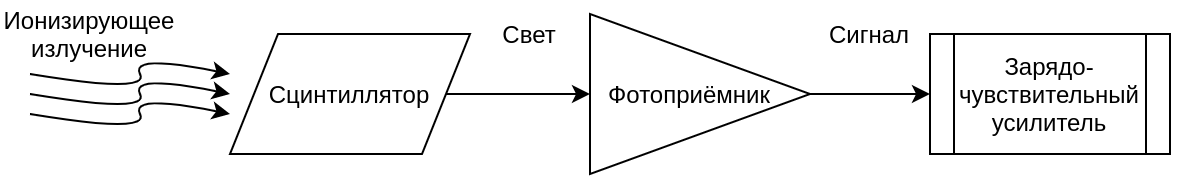
\includegraphics[width=1\linewidth]{Scintillation_detector.png}
    \caption{Схема сцинтилляционного детектора}
    \label{fig:mpr}
\end{figure}
Фотоприёмник преобразует излучённую кристаллом световую вспышку в импульс электрического тока. Полученный сигнал принимается ЗЧУ, который преобразует электрический ток в заряд. По его величине можно восстановить количество энегрии, потраченной сцинтиллятором на высвечивание за определённое время.


\section{Установка стенда по исследованию сцинтилляционных кристаллов}
    Блок-схема установки изображена на рисунке().\par
    \begin{figure}[ht]
        \centering
        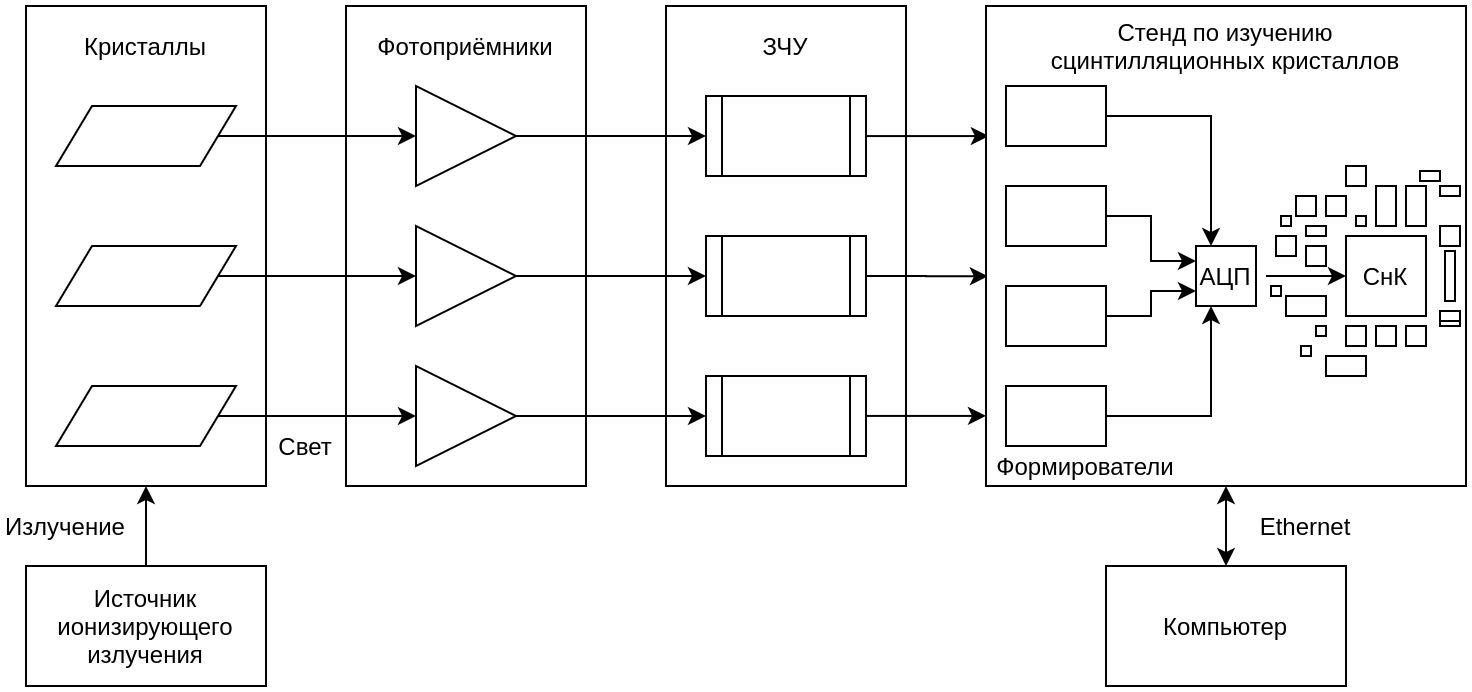
\includegraphics[width=1\linewidth]{Experimental_setup.png}
        \caption{Блок-схема установки}
        \label{fig:mpr}
    \end{figure}
    Ионизирующее излучение с источника попадает на три сцинтилляционных кристалла: исследуемый и два вспомогательных. Излучаемые кристаллами фотоны регистрируются в фотоприёмниках и преобразуются в электрические сигналы. После услиения в зарядо-чувствительных усилителях сигналы подаются на входные каналы стеда, где они обрабатываются. Результат обработки отправляется на компьютер оператора через интерфейс Ethernet. Стенд имеет, кроме основного канала, предназначенного для исследуемого кристалла, два дополнительных для вспомогательных кристаллов.
    
    \subsection{Схема стенда}
    На рисунке() представлена блок-схема стенда.\par
\begin{figure}[ht]
    \centering
    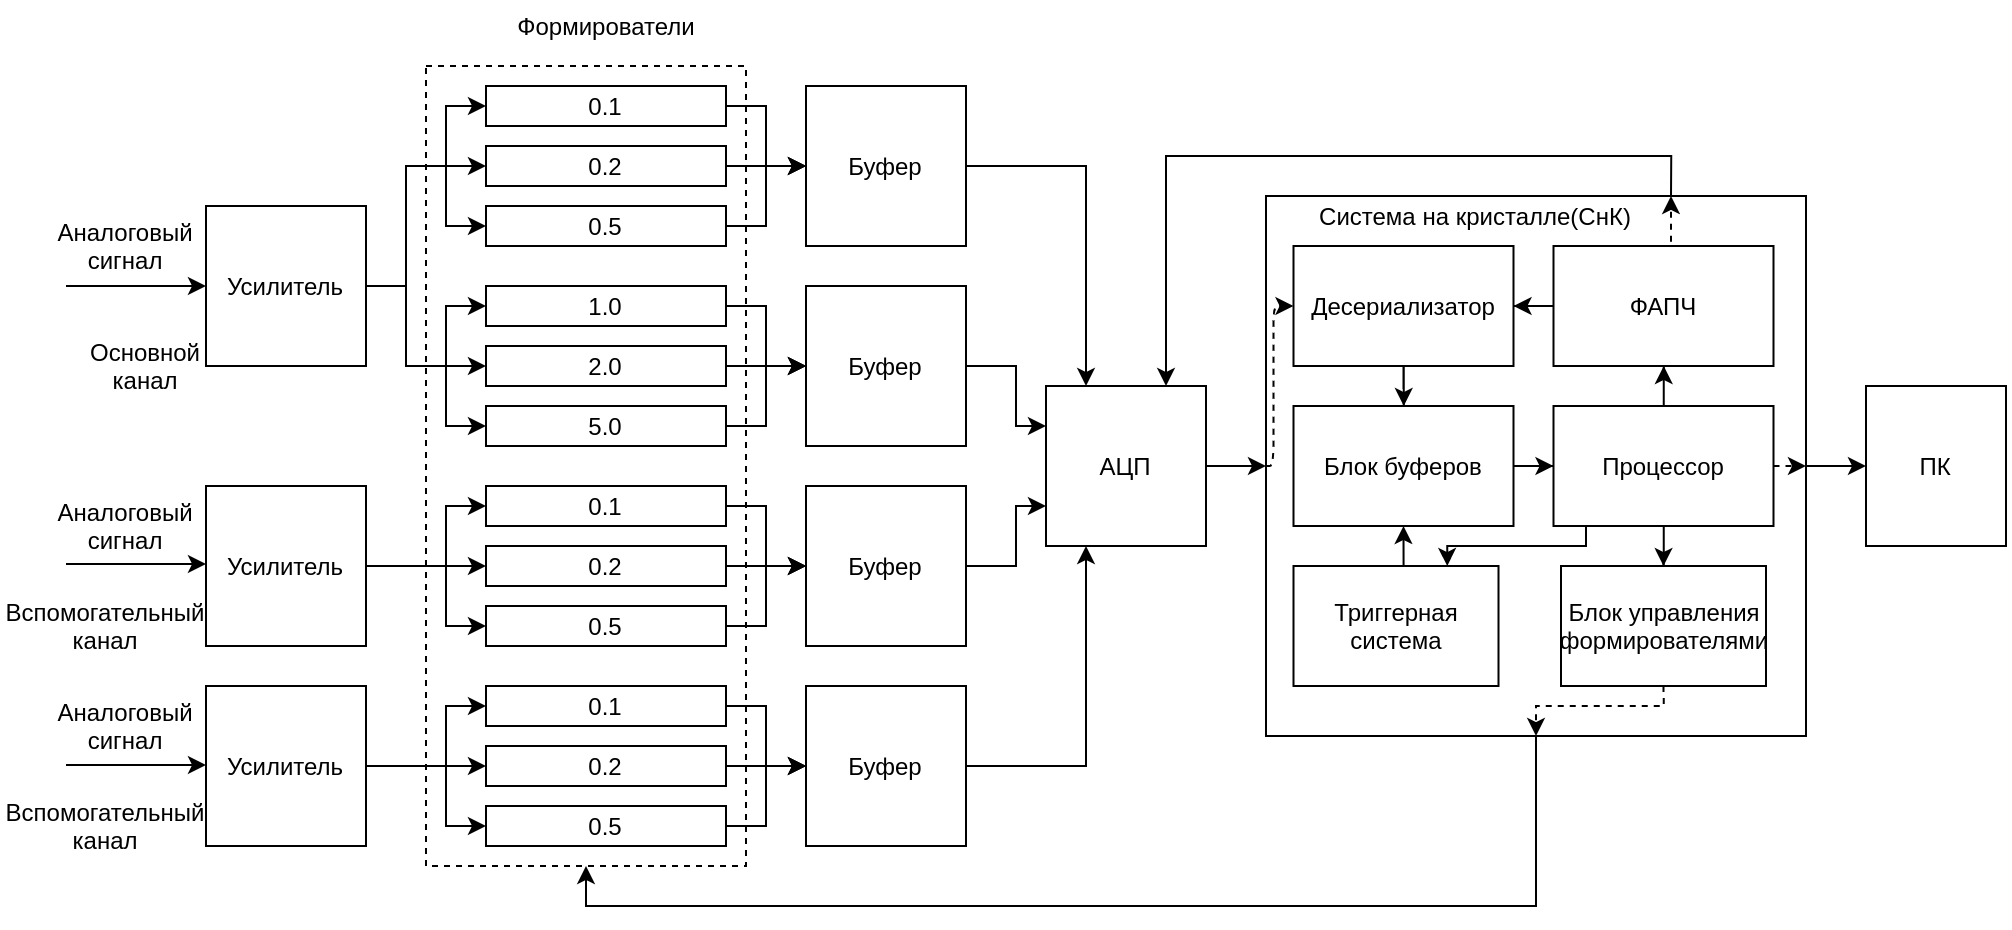
\includegraphics[width=1\linewidth]{board_scheme.png}
    \caption{Блок-схема стенда}
    \label{fig:mpr}
\end{figure}
Как было сказано выше, стенд имеет 3 входных канала: основной и 2 вспомогательных. На каждом из них предусмотрен усилитель, сигнал с которого в набор формирователей, определяющих время формирования сигнала. Далее через промежуточный буфер с дифференциальным выходом сигнал поступает в 14-битный АЦП, где происходит его конвертация в цифровой вид. Оцифровка происходит на тактовой частоте 125 МГц, выдаваемой модулем фазовой автоподстройки частоты (ФАПЧ), реализованным в системе на кристалле. Цифровые данные в последовательно упакованном формате передаются в СнК, где проводится их обработка. В первую очередь, происходит обратная конвертация из последовательности бит в число (десериализация), после чего, при срабатывании триггерной системы, данные из блока буферов отправляются в процессор для последующей обработки. Для связи с компьютером используется протокол Ethernet.\par

На рисунке () представлена фотография стенда с выделением основных блоков:\par
\begin{enumerate}
    \item Блок питаний;
    \item Система на кристалле Zynq-7000 с необходимой переферией;
    \item 4-х канальный АЦП;
    \item Формирователи основного и вспомогательных каналов
    \item Усилители сигналов;
    \item Входные разъёмы. 
\end{enumerate}

\begin{figure}[ht]
    \centering
    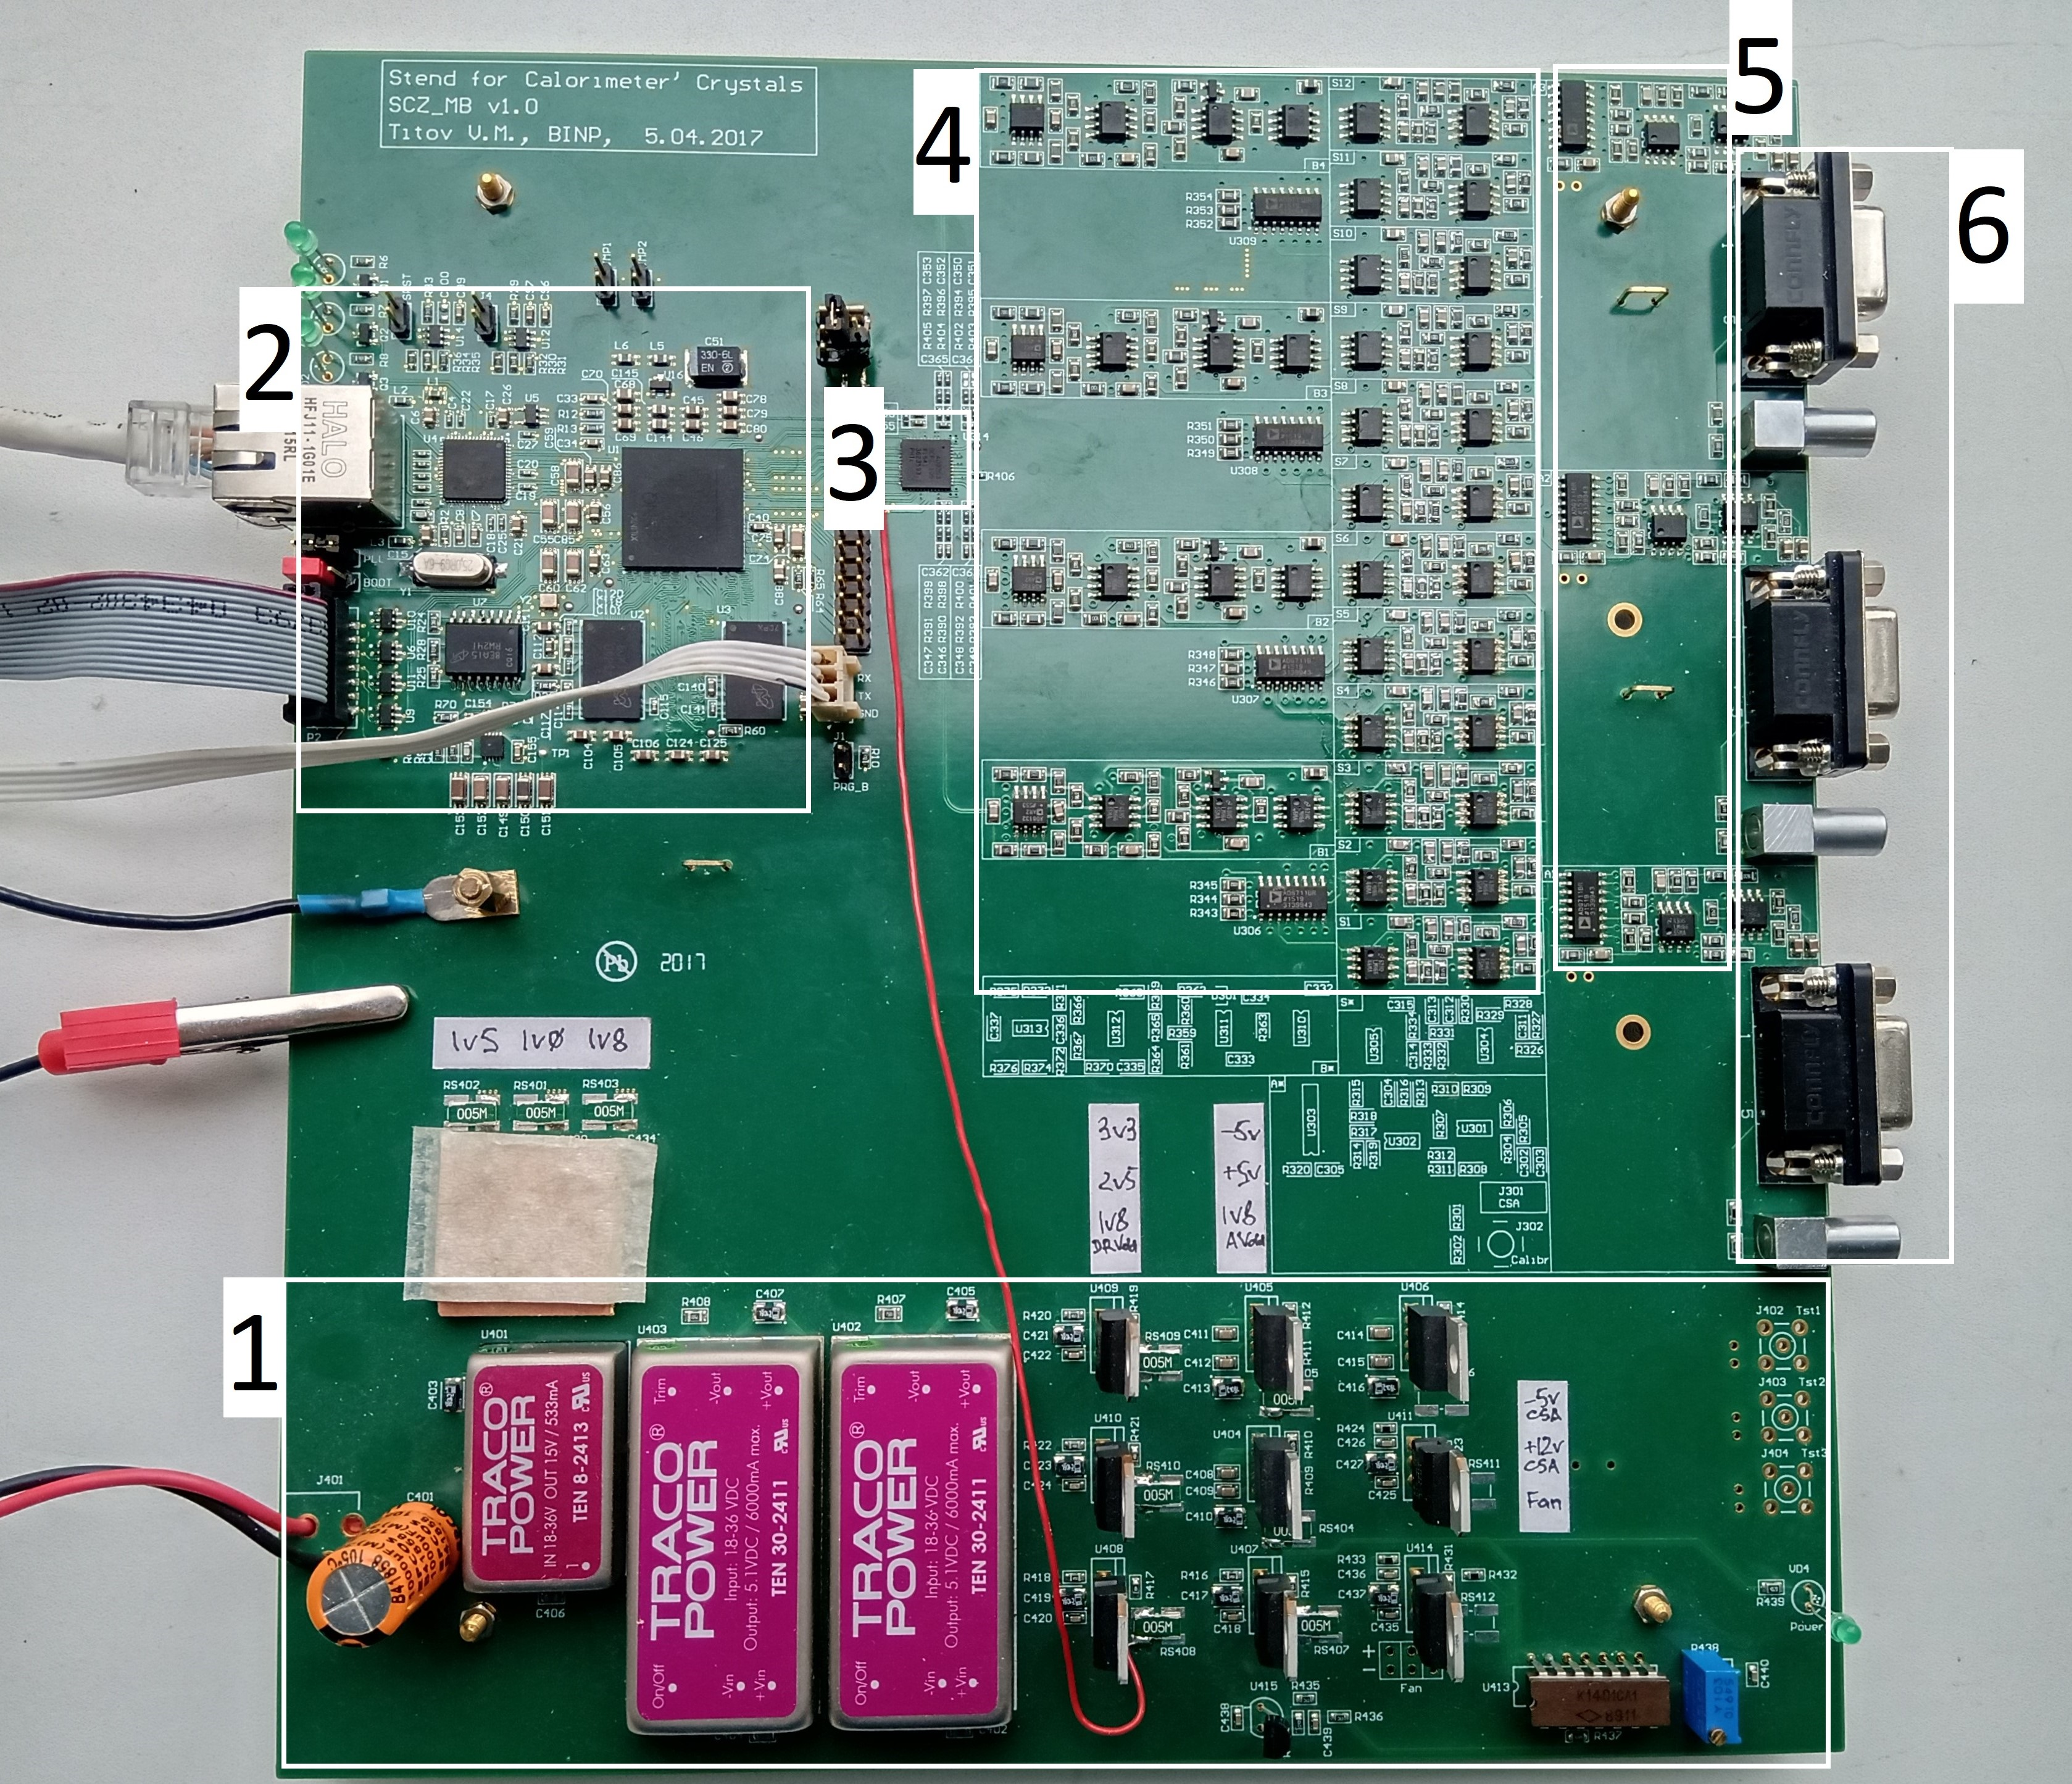
\includegraphics[width=1\linewidth]{board.jpg}
    \caption{Фотография стенда}
    \label{fig:mpr}
\end{figure}

Далее будут рассмотренны подробнее особенности устройства некоторых частей описанной системы.\par
\textbf{Основной канал}\par
Основной канал имеет 2 набора формирователей с различными временами формирования: 0.1, 0.2, 0.5 и 1, 2, 5 мкс соответственно. Данные временные значения формирователей подобраны на основе анализа свойств сцинтилляционных кристаллов, а так же имеющегося опыта работы с ними. Такие времена способны обеспечить корректную работу с большим набором кристаллов: от со сравнительно малыми временами высвечивания до больших.\par
После каждого формирователя установлены электронные ключи, с помощью которых можно подключить выход одной секции из набора через буфер ко входу АЦП. На основном канале, таким образом, имеется возможность подключить одновременно 2 формирователя из диапазона 0.1 - 0.5 и 1 - 5 мкс соответственно. Оцифрованные данные непрерывно записываются в кольцевой буфер, откуда они могут быть выгружены для обработки и сохранения при поступлении команды о полезном событии от триггерной системы.\par
\textbf{Вспомогательные каналы}\par
Вспомогательные каналы служат источниками дополнительных сигналов, необходимых для правильной работы триггерной системы. Устройство вспомогательных каналов аналогично основному во всём, кроме:\par
\begin{itemize}
    \item каждый из них содержит только по одному набору формирователей с тремя секциями с временами 0.1, 0.2, и 0.5 мкс;
    \item к аналогово-цифровому преобразователю может быть подключен выход только одной секции формирования канала.
\end{itemize}\par
\textbf{Триггерная система}\par
Триггерная система выполняет задачу формирования сигнала, означающего возникновение полезного события, при котором данные из кольцевого буфера необходимо выгрузить для последующей обработки. Система может работать в двух режимах: принудительный старт и срабатывание по порогу. В первом случае триггерная система вырабатывает сигнал при получении команды от оператора. Во втором случае триггер срабатывает при превышении текущими цифровыми значениями основного и/или некоторых вспомогательных каналов заданных оператором порогов.


\section{Дизайн системы на кристалле}
    \subsection{Процессорная система}
    Для разработки процессорной системы существуют готовые блоки, предоставляемые компанией-производителем Xilinx. В данной работе используются некоторые из них. Также для передачи команд и параметров оператора был разработан пользовательский блок виртуальных регистров. Список всех блоков и их краткое описание представлены в таблице~1.\par%\ref{tab:PS_blocks}.\par
\begin{table}[ht]
    \label{tab:PS_blocks}
    \caption{Блоки дизайна процессорной системы}
    \begin{tabular}{|p{0.45\textwidth}|p{0.5\textwidth}|}
        \hline
        Наименование блока & Описание \\
        \hline
        Процессорная система ZYNQ7 Processing System \parencite{ZYNQPS} & Программный интерфейс вокруг процессорной системы платформы Zynq-7000 \\
        \hline
        Контроллер блоков памяти AXI BRAM Controller \parencite{AXIBRAMctrl} & Является конечным ведомым модулем для интеграции с интерфейсом шины AXI и системными главными устройствами для связи с локальными блоками оперативной памяти \\
        \hline
        Интерфейс шины AXI Interconnect \parencite{AXIInterconnect} & Соединяет один или более AXI устройств, отображенных на память в режиме мастера, к одному или более устройствам, отображённых на память в режиме ведомого \\
        \hline
        Сброс процессорной системы Processor System Reset \parencite{PSReset} & Обеспечивает индивидуальные сбросы для всей процессорной системы, включая процессор и периферийные устройства \\
        \hline
        Интерфейс модуля виртуальных регистров reg\_interface & Пользовательский блок, использующий интерфейс AXI4-Lite \\
        \hline
        Генератор блоков памяти Block Memory Generator \parencite{Blockmemgen} & Автоматизирует создание блочных запоминающих устройств для программируемой логики\\
        \hline
    \end{tabular}
\end{table}
Как видно из приведённой таблицы, в процессорной системе используется несколько готовых блоков от компании Xilinx и один пользовательский модуль, который имеет смысл рассмотреть подробнее. Он разработан с использованием AXI4-Lite. Данного интерфейса хватает для корректной работы модуля в силу небольшого объёма данных, передаваемых за одну транзакцию. Задача блока \texttt{reg\_interface} заключается в передаче коротких параметров, команд и сигналов подтверждения из процессора в программируемую логику. Сигналы модуля представлены на рисунке \ref{fig:reg_interface}.\par 
\begin{figure}[ht]
    \centering
    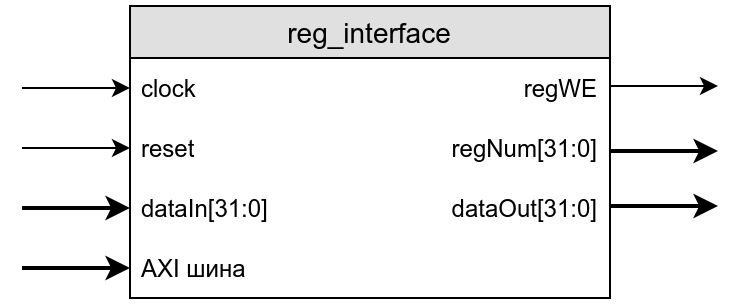
\includegraphics[width=0.5\linewidth]{reg_interface.png}
    \caption{Сигналы блока reg\_interface}
    \label{fig:reg_interface}
\end{figure}
Каждый пользовательский сигнал (\texttt{dataPLtoPS}, \texttt{regWE}, \texttt{regNum}, \texttt{dataPStoPL}) ассоциирован с определённым участком в памяти, таким образом, текущее значение по выбранному адресу является состоянием сигнала. Блок связан с модулем \texttt{reg\_file} программируемой логики, подробное описание которого будет приведено в соответствующей главе. Сейчас важно то, что этот модуль содержит виртуальные регистры, операции с ними осуществляются посредством рассматриваемого модуля \texttt{reg\_interface}, который переводит их в операции с реально существующими регистрами.\par
Для записи в виртуальный регистр необходимо вставить данные в сигнал \texttt{dataPStoPL}, затем установить номер регистра в сигнал \texttt{regNum}, после чего подать единицу в сигнал \texttt{regWE}.\par
Для чтения из виртуального регистра необходимо установить номер интересующего регистра в сигнал \texttt{regNum}, после считать данные из сигнала \texttt{dataPLtoPS}.\par
Общая диаграмма блоков процессорной системы изображена на рисунке \ref{fig:ps_top}.\par
\begin{figure}[ht]
    \centering
    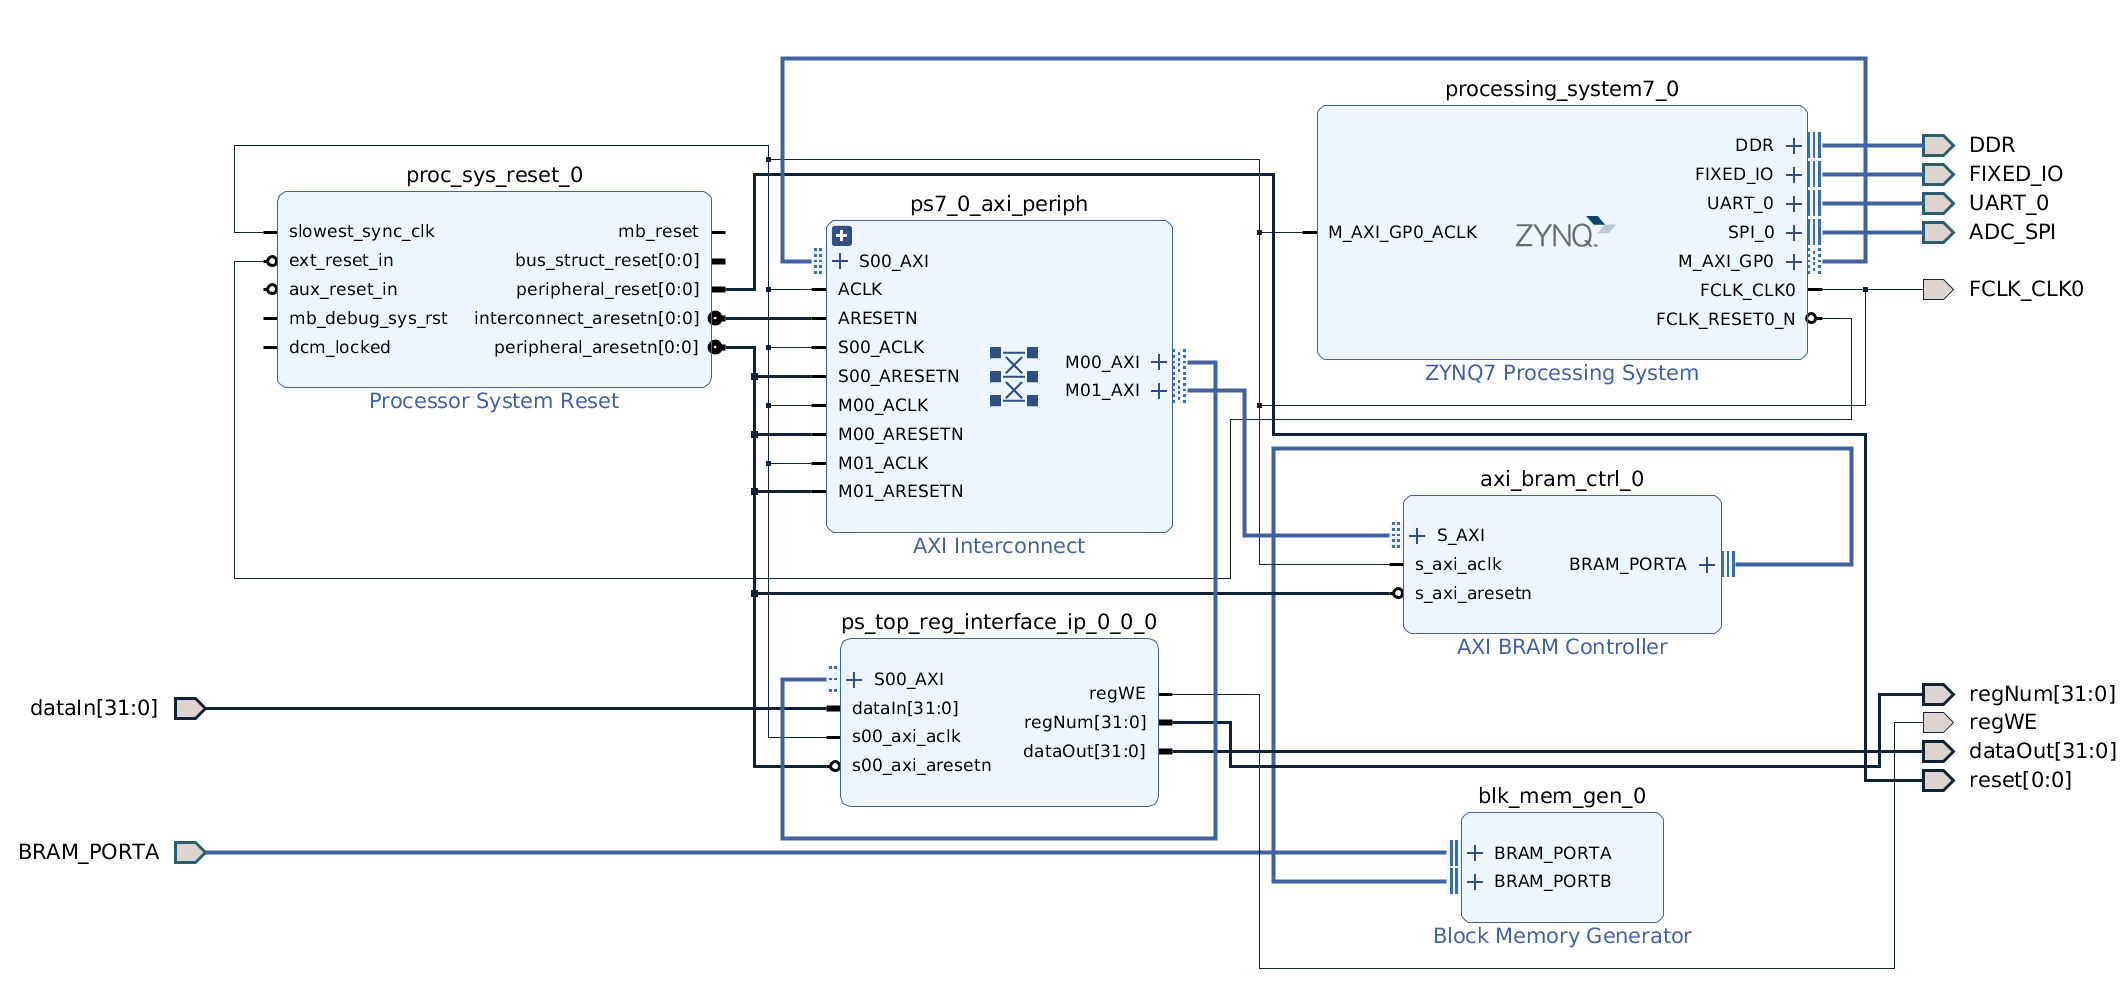
\includegraphics[width=1\linewidth]{ps_top.jpg}
    \caption{Диаграмма блоков процессорной системы}
    \label{fig:ps_top}
\end{figure}
Кроме интерфейса виртуальных регистров, рассмотренного выше, для обмена данными между процессорной системой и программируемой логикой используется модуль двухпортовой памяти \texttt{blk\_mem\_gen\_0}: через порт A происходит запись данных из программируемой логики, а через порт B информация считывается и отправляется в процессор. Настоящий модуль предназначен для передачи данных осциллограмм для их последующего отображения оператору стенда. Схожий блок двухпортовой памяти, необходимый для передачи статистических данных гистограмм расположен в части программируемой логики. Для их интеграции с интерфейсом шины AXI в процессорной системе предусмотрены контроллеры блоков памяти \texttt{oscillograms\_bram\_ctrl} и \texttt{spectra\_bram\_ctrl} соответственно.\par


    \subsection{Программируемая логика}
    На рисунке() представлена схема программируемой логики.\par 
\begin{figure}[ht]
    \centering
    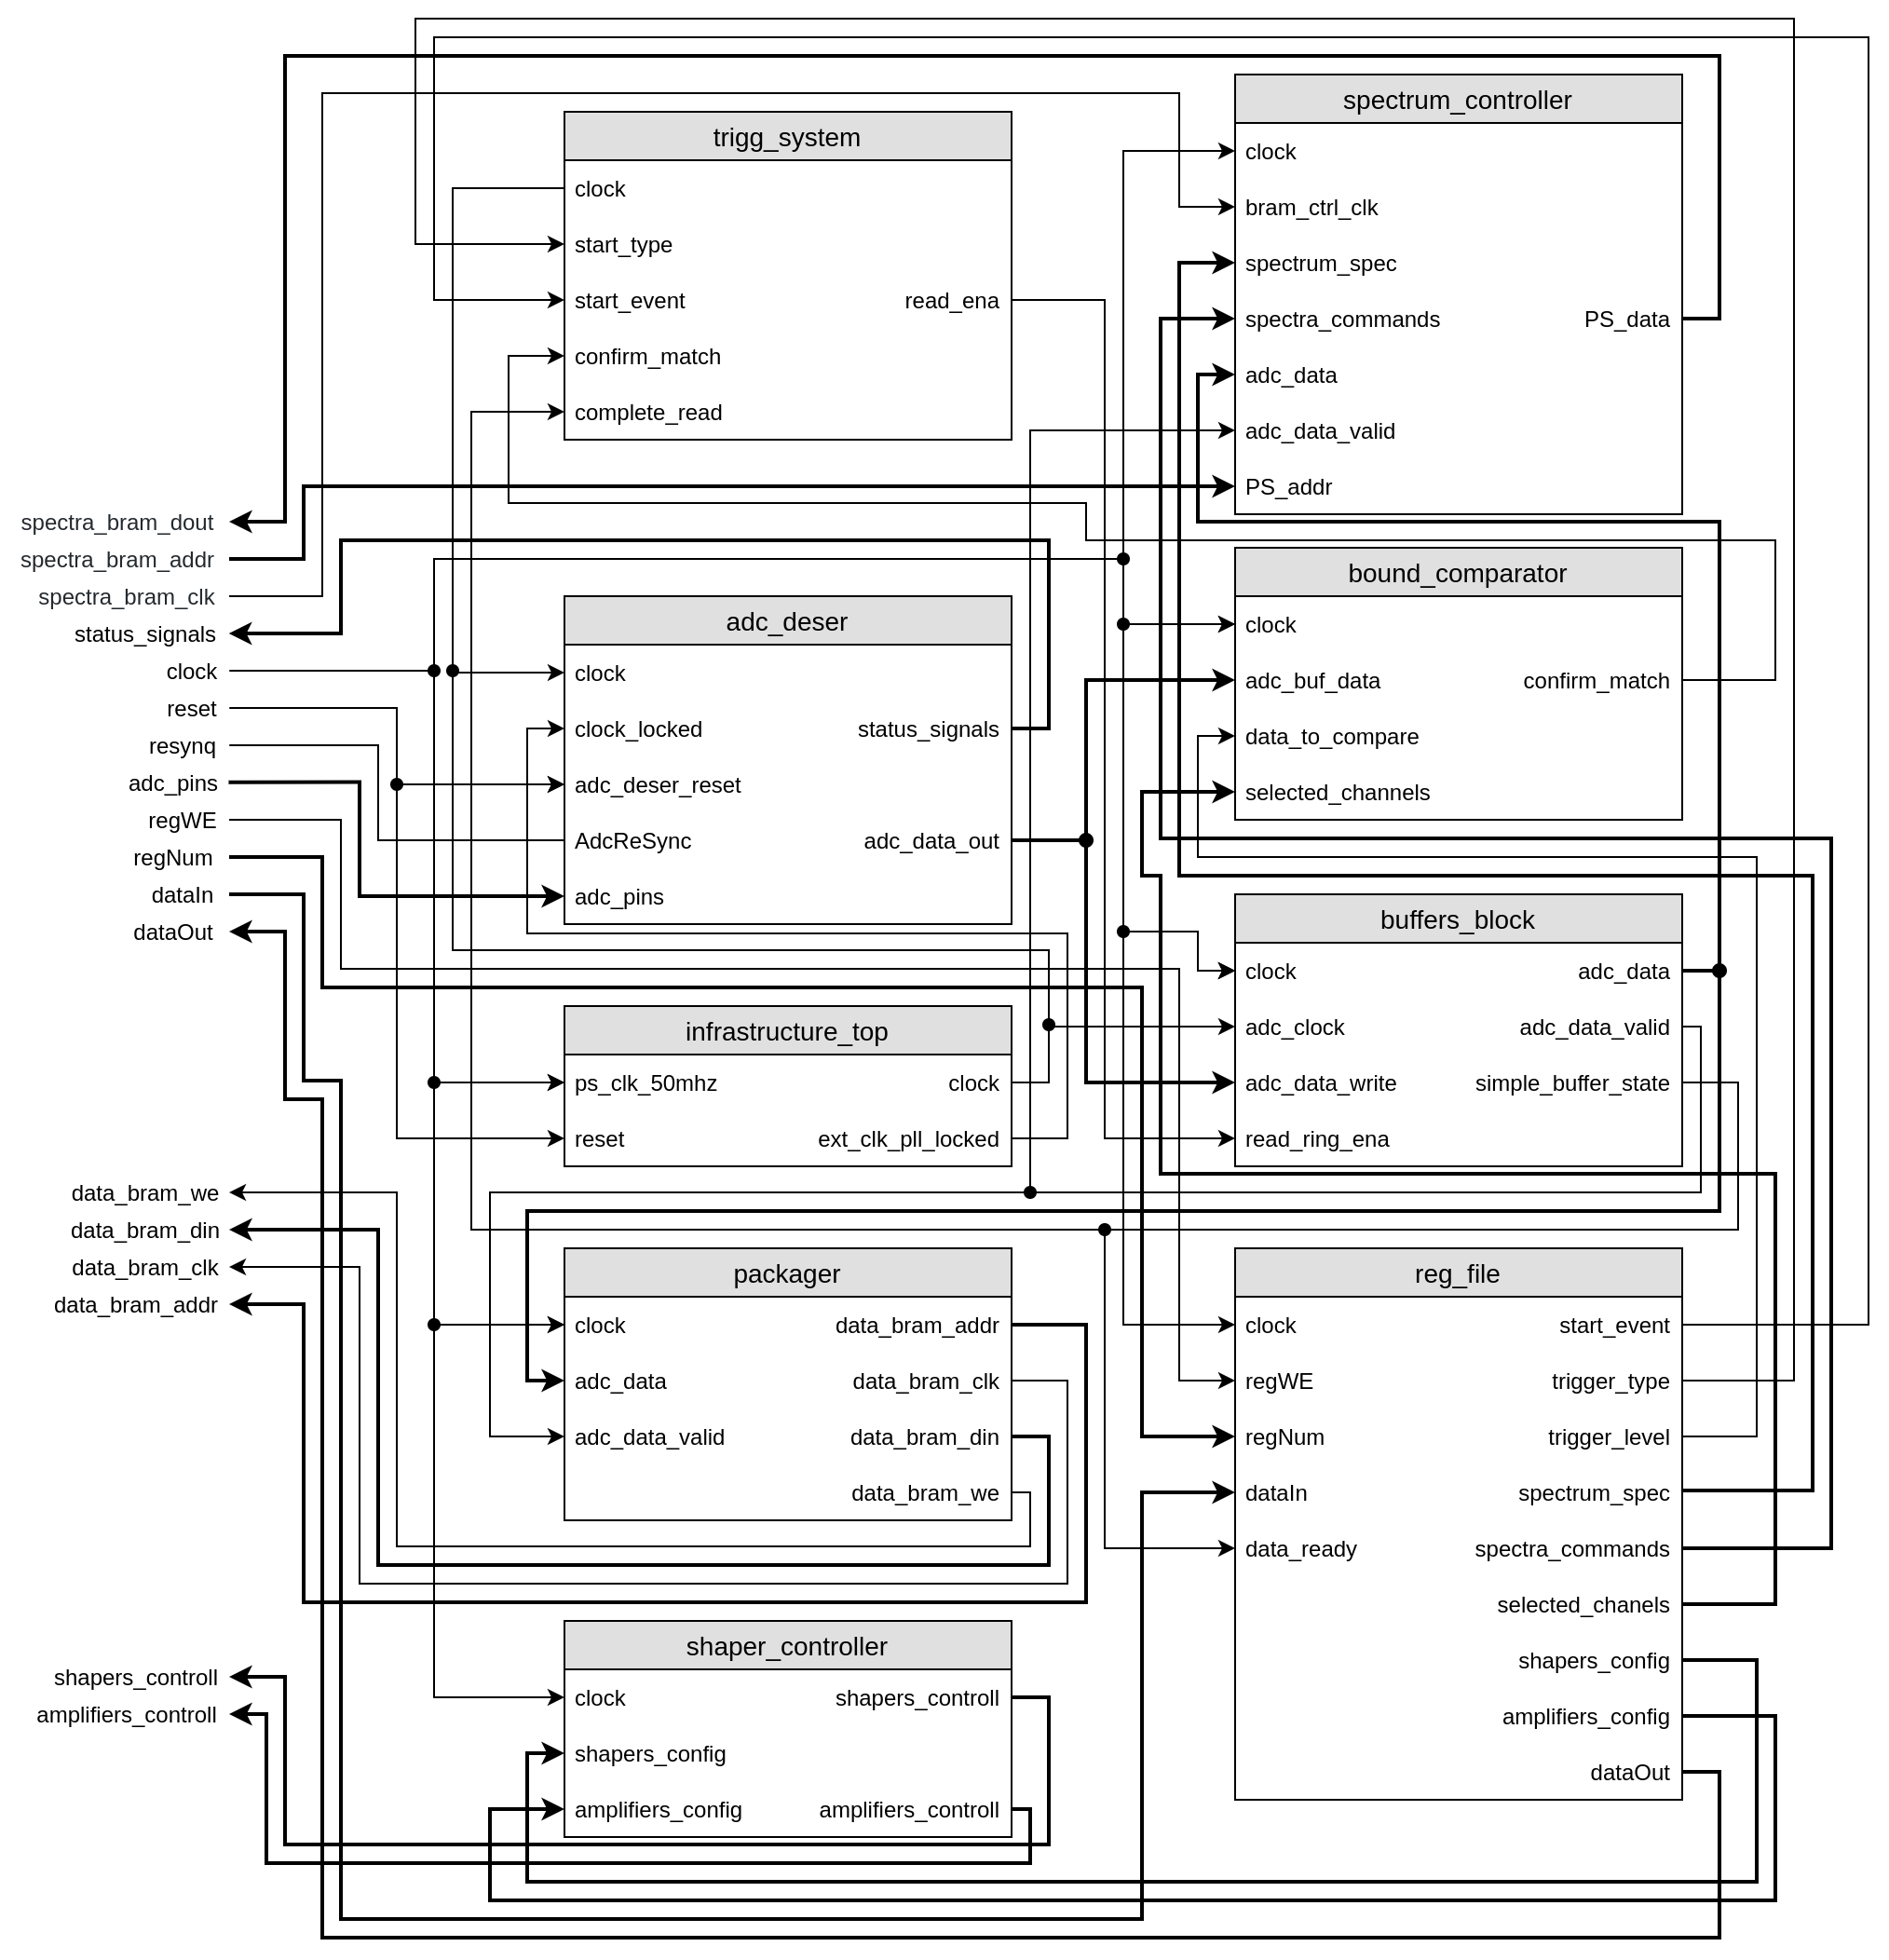
\includegraphics[width=1\linewidth]{PL_top.png}
    \caption{Блок-схема установки}
    \label{fig:mpr}
\end{figure}
Программируемая логика состоит из 9 блоков, краткое описание который представлено в таблице()\par
\begin{table}[h!]
    \caption{Блоки программируемой логики}
   % \begin{tabular}{|>{\centering\arraybackslash}p{0.45\textwidth}|>{\centering\arraybackslash}p{0.45\textwidth}|}
    \begin{tabular}{|p{0.45\textwidth}|p{0.5\textwidth}|}
        \hline
        Наименование блока & Описание \\
        \hline
        adc\_deser & Конвертирует упакованные последовательно данные АЦП в численные значения \\
        \hline
        infrastructure\_top & Обеспечивает тактовую частоту для некоторых модулей \\
        \hline
        buffers\_block & Буферизует входные данные \\
        \hline
        trigg\_system & Генерирует сигнал для сохранения данных \\
        \hline
        bound\_comparator & Выполняет сравнение входящих данных с заданными порогами \\
        \hline
        spectra\_controller & Производит обработку данных для набора статистики \\
        \hline
        shaper\_controller & Осуществляет управление формирователями сигналов \\
        \hline
        reg\_file & Реализует блок виртуальных регистров \\
        \hline
        packager & Упаковывает данные и передаёт их в процессорную систему \\
        \hline
    \end{tabular}
\end{table}
\textbf{Десериализатор adc\_deser}\par
Одним из основных элементов стенда является АЦП AD-9253. Преобразователь работает на 105 МГц параллельно в 4-х каналах. Данные с разрешением 14 бит передаются по протоколу LVDS. Этот стандарт предполагает передачу информации в последовательно-упакованном виде по 2 каналам на каждый вход. На рисунке() представлена временная диаграмма работы АЦП.\par
\begin{figure}[ht]
    \centering
    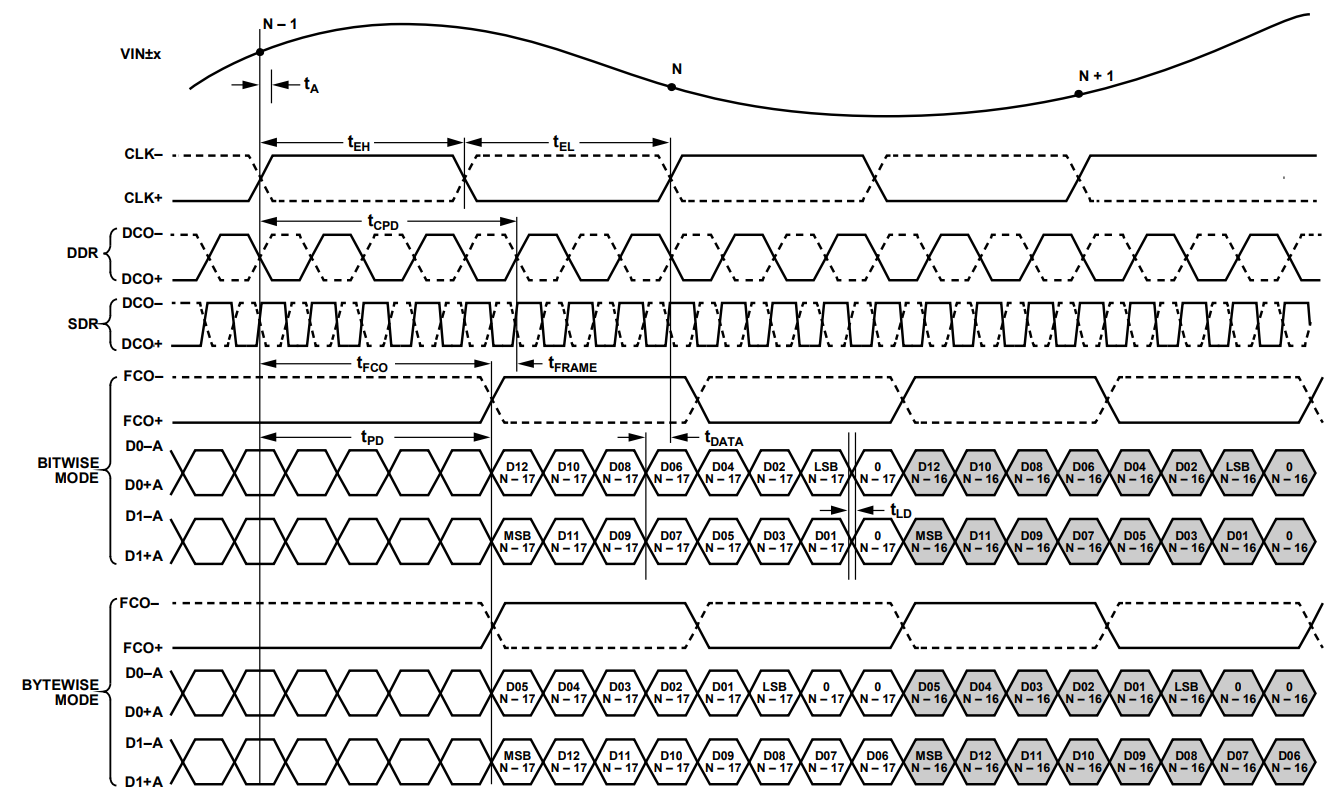
\includegraphics[width=1\linewidth]{ADC_time_diagram.png}
    \caption{Временная диаграмма работы АЦП}
    \label{fig:mpr}
\end{figure}
Каждый такт работы АЦП производится оцифровка входного аналогового сигнала. Как видно из временной диаграммы, полученные данные отправляются за 1 такт через 17 тактов после оцифровки по двум каналам. Предствляться они могут в одном из двух вариантов: побитовый (bitewise mode) и побайтовый (bytewise mode). Данные режимы отличаются последовательностью упаковки битов --- в разных каналах передаются либо четные и нечётные биты, либо младший и старший байты соответственно. В настоящей работе выбран побитовый режим, так как данные в таком виде проще обработать в программируемой логике.\par
Также в работе АЦП участвуют 2 вспомогательных сигнала --- кадровый, отвечающий за разделение набора бит на кадры оцифровки, и сигнал передачи данных, который размечает биты внутри каждого кадра.\par
Таким образом, возникает небходимость реализации модуля, осуществляющего конвертацию последовательности бит, поступающей из АЦП, в удобное для обработки численное значение. Так как процесс упаковки бит в определённую последовательность называется сериализацией, то обратную операцию можно назвать десериализаций, а соответствующий модуль --- десериализатором. Его сигналы изображены на рисунке()\par
\begin{figure}[ht]
    \centering
    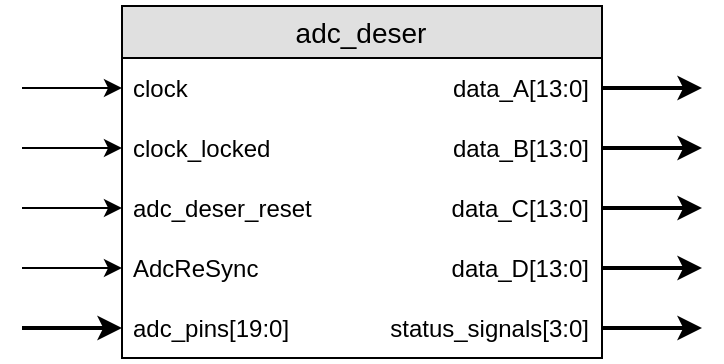
\includegraphics[width=0.5\linewidth]{adc_deser.png}
    \caption{Сигналы модуля десериализатора}
    \label{fig:mpr}
\end{figure}
Модуль был разработан ранее на основе готового интерфейса компании Xilinx, поэтому подробного описания его работы приведено не будет. Стоит лишь отметить, что входные данные принимаются через набор сигналов adc\_pins, а десериализованные значения подаются на выход через сигналы data\_i.\par
\textbf{ФАПЧ infrastructure\_top}\par
Модуль фазовой автоподстройки частоты (ФАПЧ) необходим для генерации тактового сигнала для работы АЦП и блоков, которые занимаются обработкой входных данных и их буферизацией (модули десериализатора и блока буферов). Как и десериализатор модуль ФАПЧ был разработан ранее с использованием библиотеки сложных функциональных блоков и рассматриваться подробно не будет. Сигналы модуля infrastructure\_top, в котором расположен ФАПЧ изображены на рисунке().\par
\begin{figure}[ht]
    \centering
    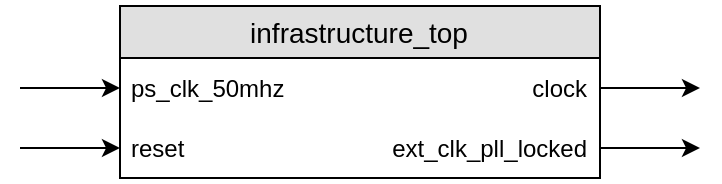
\includegraphics[width=0.5\linewidth]{infrastructure_top.png}
    \caption{Сигналы модуля infrastructure\_top}
    \label{fig:mpr}
\end{figure}
\textbf{Блок буферов buffers\_block}\par
В силу случайного характера возникновения полезных событий возникает необходимость временного хранения определённого числа последних измерений с АЦП. Для решения задачи был разработан модуль блока буферов, сигналы которого изображены на рисунке().\par
\begin{figure}[ht]
    \centering
    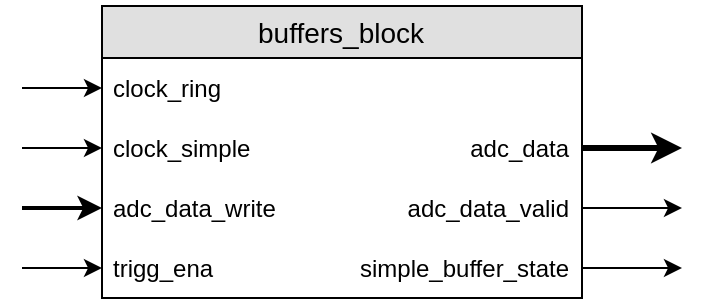
\includegraphics[width=0.5\linewidth]{buffers_block.png}
    \caption{Сигналы модуля блока буферов}
    \label{fig:mpr}
\end{figure}
Блок содежит в себе 2 модуля RAM памяти c раздельными портами чтения/записи данных. Первый является кольцевым буфером и непрерывно записывает данные с АЦП. Это позволяет сохранить некоторые данные до срабатывания триггерной системы. Такая необходимость обусловлена возможными задержками сигнала триггера, а также потербностью иметь небольшую "предысторию" осциллограммы перед достижением сигнала порогового значения.\par
Второй модуль памяти выполняет функцию простого буфера, в который временно будут выгружаться полезные данные при возникновении сигнала триггерной системы. Главной задачей такого буфера является хранение данных для гарантированного считывания и передачи их в процессорную систему.\par
Объём простого буфера определяется необходимым размером осциллограммы, который, в свою очередь, зависит от максимального времени высвечивания кристалла. Это время ограничено промежутком в 1 мкс, следовательно, учитывая частоту работы АЦП (105 Мгц), требуемый размер буфера составляет порядка 100 кадров. Для удобства объём был увеличен до 128 измерений -- осциллограмма будет подробнее, а адресация внутри буфера проще. Объём кольцевого буфера, в свою очередь, определяется максимальным колличеством данных, необходимым для восстановления. Из свойств сцинтилляционных кристаллов было принято решение об использовании 64 кадровю.\par
Модуль buffers\_block имеет два входных тактовых сигнала -- clock\_ring и clock\_simple. Система на кристалле работает на 50 МГц, следовательно, именно на этой частоте должны выгружаться данные в процессорную часть. При этом АЦП работает на 105 МГц. Здесь кроется ещё одна немаловажная задача простого буфера: переход работы с данными с одной тактовой частоты на другую. Таким образом, поток данных поступает в блок на тактовом сигнале работы АЦП, а полезная информация выдаётся на частоте работы системы на кристалле.\par
Из рисунка видно, что модуль также содержит следующие входные сигналы: adc\_data\_write -- входные данные с АЦП, trigg\_ena -- сигнал триггерной системы о возникновении полезного события. Можно заметить, что выходной набор adc\_data содержит большее число сигналов, чем входной adc\_data\_write. Это связано с добавлением к данным по 2 бита, индетифицирующих их отношение к определённому каналу. Таким образом, значение каждой оцифровки хранится ровно в двух байтах.\par
\textbf{Триггерная система trigg\_system}\par
Как было сказано ранее, для сохранения данных с АЦП в буфер и последующей их передачи в процессор необходим сигнал, сообщающий о возникновении полезного события. Генерацией такого сигнала занимается модуль триггерной системы, сигналы которого изображены на рисунке().\par
\begin{figure}[ht]
    \centering
    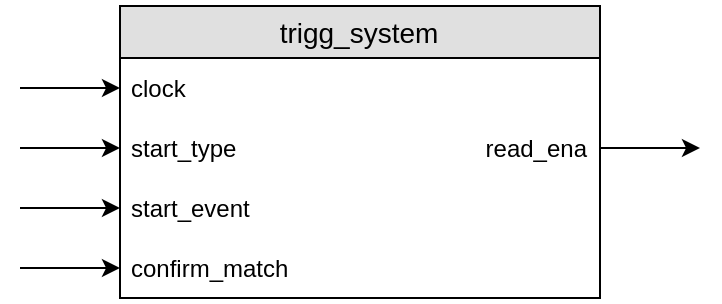
\includegraphics[width=0.5\linewidth]{trigg_system.png}
    \caption{Сигналы модуля триггерной системы}
    \label{fig:mpr}
\end{figure}
Триггерная система может работать в двух режимах, задаваемых сигналом start\_type: принудительно и по порогу. В первом случае модуль отработает сразу при появлении сигнала старта на входе start\_event. В режиме срабатывания по порогу триггер сгенерирует разрешение на запись только при появлении на входе confirm\_match высокого уровня от модуля компаратора bound\_comparator.\par
\textbf{Компаратор bound\_comparator}\par
Компаратор осуществляет сравнение текущих оцифрованных данных АЦП с заданными оператором значениями порогов. Это необходимо для корректного функционирования триггерной системы в соответствующем режиме работы. Сигналы блока изображены на рисунке()\par
\begin{figure}[ht]
    \centering
    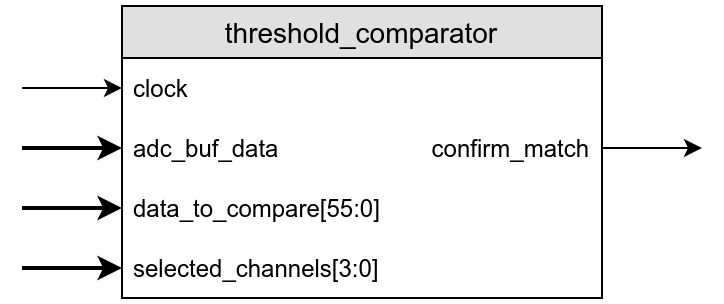
\includegraphics[width=0.5\linewidth]{bound_comparator.png}
    \caption{Сигналы модуля компаратора}
    \label{fig:mpr}
\end{figure}
Данный модуль функционирует на тактовой частоте работы АЦП, т.к. он должен непрерывно сравнивать каждое оцифрованное значение, поступающее через вход adc\_buf\_data. При достижении или превышении порогового значения модуль формирует на выходном сигнале confirm\_match логическую единицу, а в противополжном случае ноль. Порог для каждого канала задаётся отдельно с помощью сигналов data\_to\_compare. Стоит отметить, что реализована возможность выбирать каналы, выполнение условий по которым повлечёт срабатывание модуля. Оператор может назначать их в режиме логического ИЛИ: система выдаст сигнал при срабатывании компаратора хотя бы по одному из выбранных каналов. Эта информация поступает в блок компаратора через сигналы selected\_channels.\par
\textbf{Модуль набора статистики spectra\_controller}\par
\textbf{Управление блоком формирователей shapers\_controller}\par
\textbf{Модуль виртуальных регистров reg\_file}\par
\textbf{Упаковщик packager}\par


\section{Операционная система}

\section{Веб-сервер}
    \subsection{Серверная часть}
    Серверная часть разработана на языке python с использованием программной платформы Django Framework. Данные инструменты были выбраны ввиду наличия некоторых наработок для настоящей задачи. Среди достоинств такого решения можно выделить:\par
\begin{itemize}
    \item простота добавления интерпретатора языка python в файловую систему, ввиду присутствия его в пакете PetaLinux Tools;
    \item подробная документация;
    \item скорость разработки (к примеру, язык C++ избыточно сложен для веб-разработки);
    \item отсутствие необходимости в кросс-компилляции
    \item расширяемость.
\end{itemize}\par
Главной задачей сервера является реализация отправки пользовательских комманд и параметров в модуль виртуальных регистров и считывание данных из двухпортовой памяти. Для этого были разработаны обработчики HTTP запросов, а также функции для работы с регистрами и чтения данных из памяти. Для доступа к переферии использован пакет python-periphery.\par

    \subsection{Клиентская часть}
    На рисунке \ref{fig:server} представлен внешний вид пользовательского веб-интерфейса.\par
\begin{figure}[ht]
    \centering
    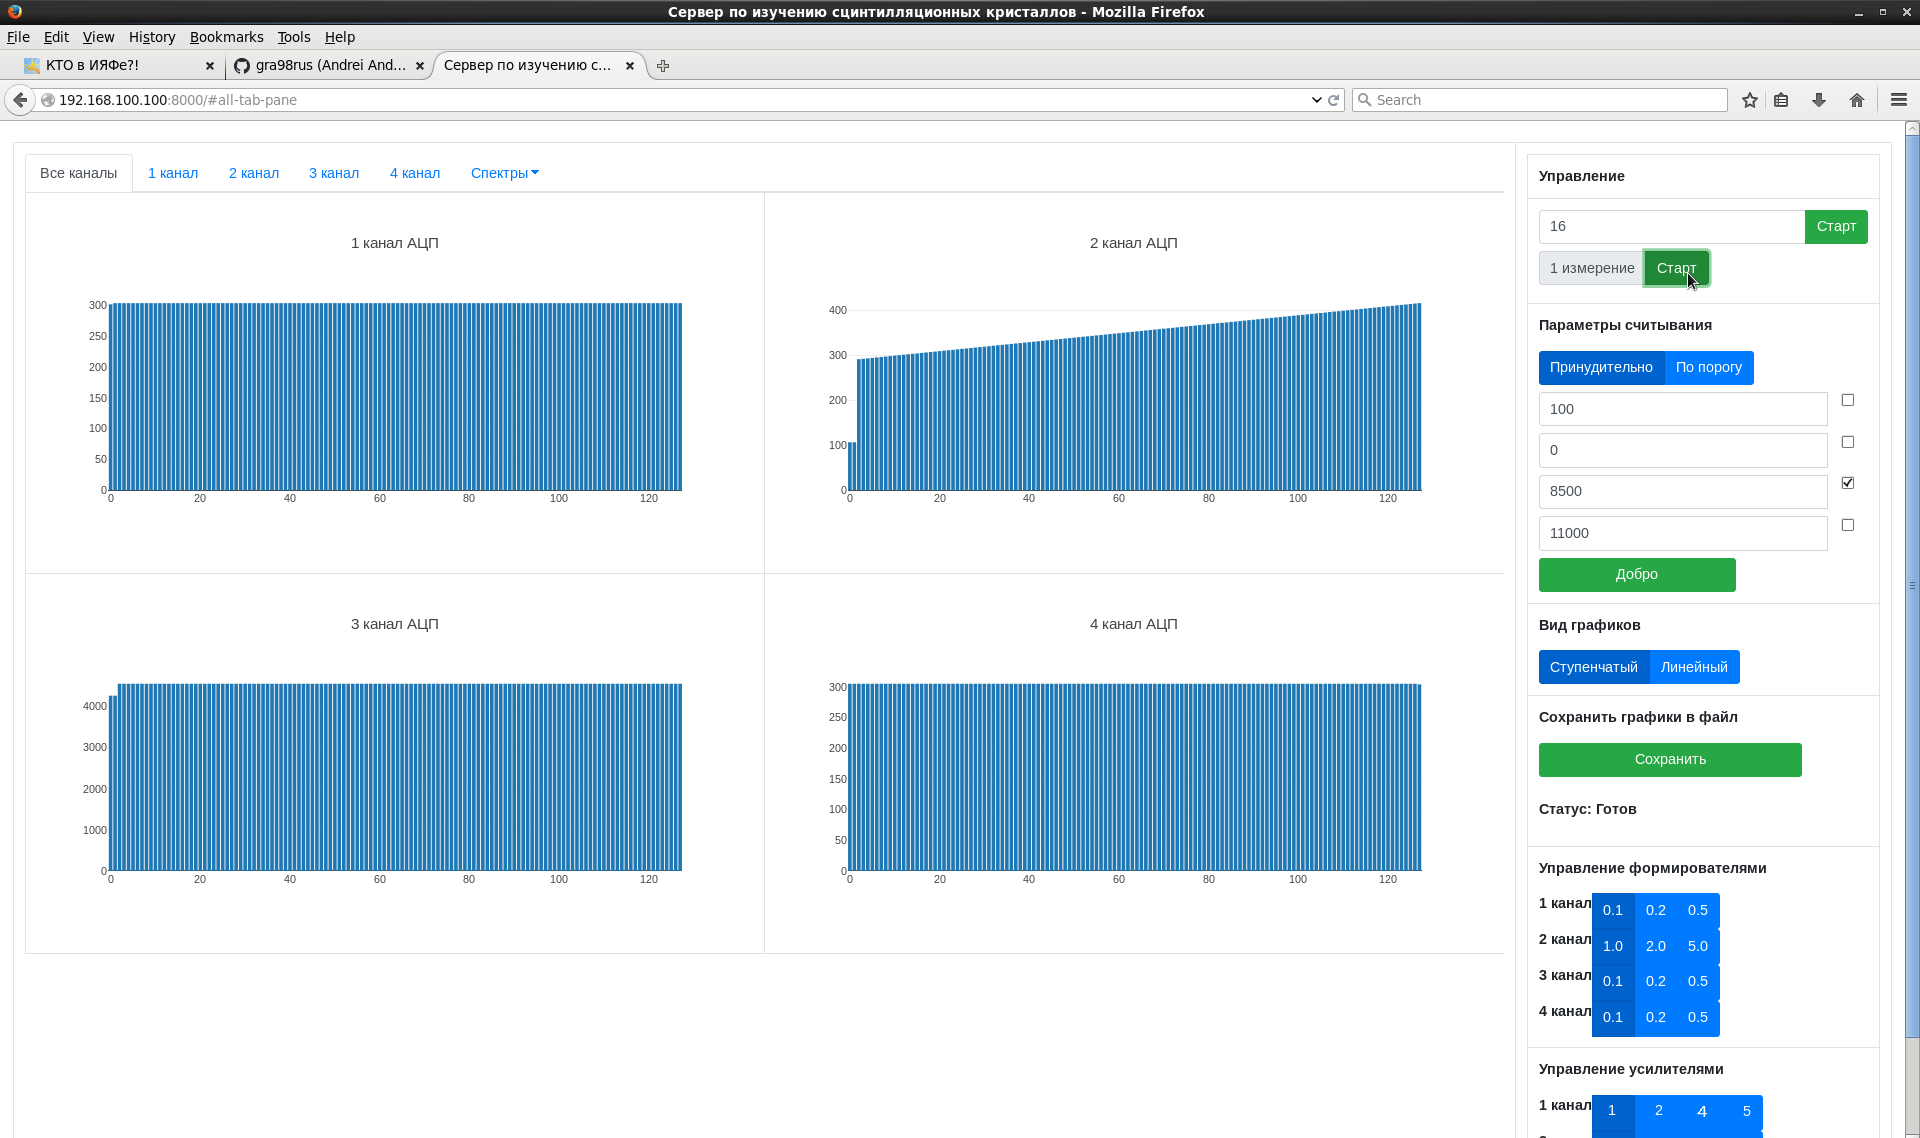
\includegraphics[width=1\linewidth]{server.jpg}
    \caption{Пользовательский веб-интерфейс}
    \label{fig:server}
\end{figure}
На главной странице расположены область с графиками и панель управления стендом. В верхней части страницы предусмотрены вкладки для переключения между графиками. Также здесь расположена вкладка ``Спектры'', где оператор может управлять гистограммами: добавить новую с выбранными параметрами или удалить существующие. Среди параметров присутствуют: выбранный канал АЦП, количество корзин (от 32 до 4096) и тип гистограммы (по максимальному значению амплитуды или же по амплитуде опорной точки, которую также можно задать).\par
На боковой панели управления оператор может задавать следующие параметры:\par
\begin{itemize}
    \item количество запусков;
    \item тип считывания (принудительный или по порогу);
    \item значения порогов для каждого канала АЦП, а также по каким каналам возможно срабатывание;
    \item вид графиков (ступенчатый или линейный);
    \item коэффициент усиления сигналов и времена формирования каждого входного сигнала.
\end{itemize}\par
Также реализована возможность сохранять данные в файл для последующего анализа.\par
Разработка велась с использованием языков JavaScript, HTML и CSS. \par


\section{Заключение}

\section{Список литературы}

\end{document}
